% ---------------------------------------------------------------------
% HEADER
% Formålet med å legge header til et eget dokument er å garantere at
% oppsettet av dokumentene er likt for alle løsningsforslagene.
% I headeren skjer følgende:
% (1) Dokumentet blir startet
% (2) Pakker blir importert
% ---------------------------------------------------------------------
% ---------------------------------------------------------------------
% HEADER
% Formålet med header er å importere de samme pakkene i alle dokumentene.
% ---------------------------------------------------------------------

% Sett opp dokumentet. Her kan 'twoside' brukes for printing
\documentclass[12pt, a4paper]{article}

% Vi trenger utf-8 for å bruke norske bokstaver: Æ, Ø, Å
\usepackage[utf8]{inputenc}

% Vi setter babel til norsk, da får dokumentegenskaper norske titler
\usepackage[norsk]{babel}

% For å kunne bruke grafikk
\usepackage{graphicx}
\newcommand{\figwidth}{0.75}

% Matematikkpakker fra AMS - American Mathematical Society
\usepackage{amsmath, amsthm, amsfonts, amssymb, mathtools}

% For eventuelle linker, e.g. \href{URL}{text}
\usepackage{hyperref}

% For headers og footers med eventuell logo
\usepackage{fancyhdr}

% Sett marginer manuelt
\usepackage[top = 3cm, left = 3cm, right = 3cm, bottom = 3cm]{geometry}

% For enkle lister, nyttig for oppgave a), b), c), ...
\usepackage[sharp]{easylist}

% Dersom flere kolonner er ønskelig i deler av dokumentet
\usepackage{multicol}

% For luft mellom paragrafer
\usepackage{parskip}

% For logikk assosiert med logoer
\usepackage{ifthen}

% For å finne totalt antall sider
\usepackage{lastpage}

% Annet
\usepackage{enumitem}

\usepackage{polynom}% Polynomer
\polyset{style=C, div=:}

\usepackage{systeme}% Likningssystemer

% Kan brukes når noe stryker ut noe, f.eks 1/n * n, her kan man ta \frac{1}{\cancel{n}} * \cancel{n}
\usepackage{cancel}



% ---------------------------------------------------------------------
% DOKUMENTVARIABLER
% ---------------------------------------------------------------------
\newcommand{\fagkode}{S2}
\newcommand{\semesteraar}{våren 2017}
\newcommand{\forfatter}{Tommy O.}
\newcommand{\dokumenttittel}{Løsningsforslag -- Eksamen \fagkode, \semesteraar}


% Set til 'true' og oppgi logo dersom du vil bruke en logo
\newboolean{bruklogo}
\setboolean{bruklogo}{true}
\newcommand{\logonavn}{figs/metis_akademiet_privatistskole_doclogo.png}

% ---------------------------------------------------------------------
% SETUP
% Formålet med å legge setup til et eget dokument å garantere at headers,
% footers, og øverste del av dokumentet er likt for alle
% løsningsforslagene.
% ---------------------------------------------------------------------
% ---------------------------------------------------------------------
% HEADER
% Formålet med setup er at dokumentene ser rimelig like ut.
% ---------------------------------------------------------------------


% ---------------------------------------------------------------------
% Alternativ font. Kommentert ut fordi Computer Modern (default) er pen
%\usepackage{kmath,kerkis}
%\usepackage[T1]{fontenc}
% ---------------------------------------------------------------------


% ---------------------------------------------------------------------
% Sett opp headers og footers
\ifthenelse{\boolean{bruklogo}}{
% Dersom logo skal brukes, sett logoen oppe til høyre med bredde 4 cm
	\rhead{\includegraphics[width=3.5cm]{\logonavn}}
}{
% Dersom logo ikke skal brukes, sett tom header
	\rhead{}
} 
\rfoot{\thepage}
\cfoot{}
\lhead{}
\lfoot{{\scriptsize Forbedringsforslag? Bidra på \url{https://github.com/tommyod/matte_eksamener_VGS}.}}
\renewcommand{\headrulewidth}{0pt}
% ---------------------------------------------------------------------


% ---------------------------------------------------------------------
% To streker under svaret
\def\answer#1{\underline{\underline{#1}}}
% ---------------------------------------------------------------------


% ---------------------------------------------------------------------
% Start selve dokumentet
% ---------------------------------------------------------------------

\begin{document}
\pagestyle{fancy}
{\bfseries \Large \dokumenttittel} \\
{ \footnotesize Laget av \forfatter 
	\hfill Sist oppdatert: \today 
	\hfill Antall sider: \pageref*{LastPage}}
\hrule
\vspace{1em}
\begin{center}
\fbox{\fbox{\parbox{.90\textwidth}{
	Dette dokumentet er open-source;
	alle kan bidra til å gjøre det bedre.
	Dersom du finner skrivefeil, matematiske feil, eller ser at forklaringene kan være bedre: ikke nøl med å sende inn en endring. 
	Du kan finne siste versjon, og bidra, på GitHub, se:
	\url{https://github.com/tommyod/matte_eksamener_VGS}
}}}
\end{center}


% ---------------------------------------------------------------------
% DOKUMENTSTART - Skriv løsningsforslaget nedenfor
% ---------------------------------------------------------------------	
\section*{Del 1 - uten hjelpemidler}
\subsection*{Oppgave 1}
\begin{easylist}[enumerate]
	\ListProperties(Style2*=,Numbers=a,Numbers1=l,FinalMark={)})
	# Vi skal derivere $f(x) = x^2 - 2/x = x^2 - 2x^{-1}$.
	Den eneste regelen vi trenger her er $\left(kx^n\right)' = knx^{n-1}$, vi får følgende utregning:
	\begin{align*}
		f'(x) &= \left(x^2\right)' - \left(2x^{-1}\right)' \\
			&= 2x - 2(-1)x^{-2} \\
			&= 2x + 2x^{-2} \\
			&= \answer{2 \left( x + \frac{1}{x^2}\right)}
	\end{align*}
	
	# Vi skal derivere $g(x) = \ln \left( x^2 + 1\right)$. Her må vi bruke kjernereglen, og vi må vite at $\left( \ln (u)\right)' = u'/u$. Vår kjerne er $u = x^2 + 1$, og $u' = 2x$. Vi får:
	\begin{align*}
	g'(x) &= \left( \ln (u)\right)' = \frac{1}{u} u' \\
	&= \frac{1}{x^2 + 1} 2x \\
	&= \answer{\frac{2x}{x^2 + 1}  }
	\end{align*}
	
	# Vi skal derivere $h(x) = x^2 e^x$. Vi må bruke produktregelen $\left(uv\right)' = u'v + uv'$ her. Velg $u = x^2$ og $v = e^x$, vi får følgende utregning:
	\begin{align*}
	g'(x) &= \left( x^2 e^x \right)' \\
	&= \left( x^2  \right)' e^x + x^2 \left( e^x\right)' \\
	&= 2x e^x + x^2 e^x \\
	&= \answer{x e^x \left(x+2\right)}
	\end{align*}
\end{easylist}

\subsection*{Oppgave 2}
I denne oppgaven skal vi se på følgende likningssystem.
\begin{align}
	\label{eq:set1} x + y -z &= 0 \\
	\label{eq:set2} 2x + y -z &= 2 \\
	\label{eq:set3} 4x + y -2z &= 1 
\end{align}
Det er lurt å bruke litt tid på å kikke på likningssystemet. Det er mange mulige måte å løse 
et slikt system på, men på eksamen er oppgavene ofte konstruert på en måte slik at enkelte
strategier er mye raskere enn andre.
Vi tar likning \eqref{eq:set2} og trekker fra likning \eqref{eq:set1}. Da får vi at $\answer{x = 2}$.
Deretter setter vi $x = 2$ inn i likning \eqref{eq:set2} og likning \eqref{eq:set3}, slik at vi får følgende 2 likninger:
\begin{align}
\label{eq:set4}  y -z &= -2 \\
\label{eq:set5} y -2z &= -7
\end{align}
Vi tar likning \eqref{eq:set4} minus likning \eqref{eq:set5} og finner at $\answer{z = 5}$. 
Nå kan vi sette inn $x$ og $z$ i hvilken som helst likning for å finne at $\answer{y = 3}$.
På eksamen bør du sette prøve på svaret for å sjekke at det stemmer.


\subsection*{Oppgave 3}
\begin{easylist}[enumerate]
	\ListProperties(Style2*=,Numbers=a,Numbers1=l,FinalMark={)})
	# Generelt så har vi at $a_n = a_1 + d(n-1)$ i en aritmetisk rekke. Vi setter inn $a_1 = 3$ og $a_6 = 18$ og
	får følgende likning:
	\begin{equation*}
		a_n = a_1 + d(n-1) \quad \Rightarrow \quad 18 = 3 + d(6-1).
	\end{equation*}
	Da finner vi ut at $\answer{d = 3}$. Vi setter dette inn i likningen ovenfor, og får følgende likning for $a_n$:
	\begin{equation*}
		\answer{a_n = 3 + 3(n-1) = 3n}
	\end{equation*}
	
	# Generelt er summen av de $n$ første leddene i en aritmetisk rekke gitt ved:
	\begin{equation*}
		S_n = \frac{\left(a_1 + a_n\right)n}{2}
	\end{equation*}
	Vi setter inn $a_1 = 3$, $a_n = 3$ og får:
	\begin{equation*}
		S_n = \frac{\left(a_1 + a_n\right)n}{2} = \frac{\left(3 + 3n\right)n}{2} = 
		\frac{3\left(1 + n\right)n}{2} = \answer{\frac{3}{2} n \left(n+1\right)}
	\end{equation*}
	Dette stemmer overens med det oppgaven ba oss om å vise.
	
	# Dersom summen skal være $84$ får vi følgende likning basert på forrige deloppgave:
	\begin{equation*}
		84 = \frac{3}{2} n \left(n+1\right) \Leftrightarrow n^2 + n - 56 = 0
	\end{equation*}
	Vi kan løse $n^2 + n - 56 = 0$ ved å gjette, eller ved å bruke ABC-formelen. Dersom vi bruker ABC formelen får vi at
	\begin{equation*}
		n_{1,2} = \frac{-1 \pm \sqrt{1 - 4 (-56)}}{2} = \frac{-1 \pm \sqrt{225}}{2} = 
		\frac{-1 \pm 15}{2} = \answer{7}
	\end{equation*}
	Legg merke til at vi ser bort i fra det negative svaret her; det gir ikke mening i forhold til denne oppgaven.
\end{easylist}

\subsection*{Oppgave 4}
I denne oppgaven skal vi se på tredjegradspolynomet $f(x) = x^3 + 4x^2 + x - 6$.
\begin{easylist}[enumerate]
	\ListProperties(Style2*=,Numbers=a,Numbers1=l,FinalMark={)})
	# Dersom $f(1) = 0$ så er $x = 1$ et nullpunkt. Da er $(x-1)$ en faktor.
	Vi utfører polynomdivisjonen $f(x) : (x-1) = \left(x^3 + 4x^2 + x - 6\right): (x-1)$
	og får $x^2 + 5x + 6$ som svar. Vi faktoriserer $x^2 + 5x + 6 = (x+2)(x+3)$
	ved hjelp av ABC-formelen, eller ved hjelp av en annen metode.
	Uansett fremgangsmåte finner vi ut at faktoriseringen blir:
	\begin{equation*}
		f(x) = x^3 + 4x^2 + x - 6 = \answer{(x-1)(x+2) (x+3)}
	\end{equation*}
	Dersom svaret ikke allerede var gitt i oppgaveteksten ville det nok ha vært lurt å sjekke at faktoriseringen stemmer ved å gange sammen faktorene og
	se at du får $x^3 + 4x^2 + x - 6$. Det går rimelig fort og gir en ekstra sikkerhet på eksamen.
	
	# For å løse $f(x) \leq 0$ setter vi opp en fortegnslinje som vist på figur \ref{fig:fortegn} nedenfor.
	\begin{figure}[th!]
		\centering
		
\includegraphics[width=0.65\linewidth]{figs/fortegn.pdf}
		\caption{Fortegnslinje til oppgave 4b, del 1.}
		\label{fig:fortegn}
	\end{figure}

	Fra figuren ser vi at \answer{$f(x) \leq 0$ når $x \leq -3$ eller når $-2 \leq x \leq 1$}.
	# Vi bruker faktoriseringen $x^3 + 4x^2 + x - 6 = (x-1)(x+2) (x+3)$
	fra den første deloppgaven, og at $2x^2 - 2 = 2 (x^2 - 1) = 2(x+1)(x-1)$. Vi får:
	\begin{equation*}
		\frac{x^3 + 4x^2 + x - 6}{2x^2 - 2} = \frac{(x-1)(x+2) (x+3)}{2(x+1)(x-1)} = \answer{\frac{(x+2) (x+3)}{2(x+1)}}
	\end{equation*}
	
	# Tidligere viste vi at $y^3 + 4y^2 + y - 6 = (y-1)(y+2) (y+3)$.
	Med andre ord har likningen $(y-1)(y+2) (y+3) = 0$ løsningene $y = 1$, $y = -2$ og $y = -3$.
	Vi skriver $e^x$ om til $y$ slik som dette:
	\begin{align*}
		e^{3x} + 4e^{2x} + e^{x} - 6 &= 0 \\
		\left(e^x\right)^3 + 4\left(e^x\right)^2 + \left(e^x\right) - 6 &= 0 \\
		y^3 + 4y^2 + y - 6 &= 0
	\end{align*}
	De mulige løsningene er $y = e^x = 1$, $y = e^x = -2$ og $y = e^x = -3$.
	Ettersom eksponentialfunksjonen alltid er positiv\footnote{At eksponentialfunksjonen alltid er positiv er grunnen til at vi ikke kan ta logaritmen av et negativt tall.} er $e^x = 1$
	den eneste mulige løsningen, som vi derfor beholder. Da er $\answer{x = 0}$ vårt endelige svar.
\end{easylist}

\subsection*{Oppgave 5}
\begin{easylist}[enumerate]
	\ListProperties(Style2*=,Numbers=a,Numbers1=l,FinalMark={)})
	# Vi deriverer og setter inn $x = 500$:
	\begin{align*}
		K'(x) = 0.2x +70 \qquad & K'(500) = 100 + 70 = 170 \\
		I'(x) = -0.1x +280 \qquad & I'(500) = -50 + 280 = 230 
	\end{align*}
	En liten positive endring i $x$ mot mer produserte enheter øker altså
	kostnaden med 170 og inntekten med 230. Vi \answer{bør produsere flere enn
	500 enheter}, fordi økningen inntekt per enheten overskrider økningen i kostnad per enhet når $x = 500$.

	# Vi deriverer overskuddet og setter lik null:
	\begin{align*}
		O(x) = I(x) - K(x) &\Rightarrow O'(x) = I'(x) - K'(x) \\
		O'(x) = 0 &\Leftrightarrow I'(x) = K'(x).
	\end{align*}
	Å finne $x$ som maksimerer $O(x)$ er det samme som å løse $I'(x) = K'(x)$.
	Vi løser $I'(x) = K'(x)$ slik som dette:
	\begin{align*}
		-0.1x +280  &=  0.2x +70 \\
		0.3 x &= 210 \\
		x &= 700
	\end{align*}
	Den vinningsoptimale produksjonsmengden er $\answer{x = 700}$.
	
	# Kostnad per enhet blir
	\begin{equation*}
		G(x) = \frac{K(x)}{x} = \frac{0.1x^2 + 70x +4000}{x} =  0.1x + 70 + \frac{4000}{x}
	\end{equation*}
	Vi må løse $G'(x) = 0$.\footnote{Vi kan også vise at $G'(x) = 0$ når $K'(x) = G(x)$, og bruke dette for å løse oppgaven.} Den deriverte blir $G'(x) = 0.1 -4000/x^2$.
	Vi løser
	\begin{equation*}
		0.1 -4000/x^2 = 0 \quad \Rightarrow \quad x = 200
	\end{equation*}
	Den kostnadsoptimale produksjonsmengden er $\answer{x = 200}$.
\end{easylist}

\subsection*{Oppgave 6}
\begin{easylist}[enumerate]
	\ListProperties(Style2*=,Numbers=a,Numbers1=l,FinalMark={)})
	# $P(X \geq 2) = P(X = 2) + P(X = 3) + P(X = 4) = 0.3 + 0.3 + 0.1 = \answer{0.7}$
	# Generelt så er forventningsverdien gitt ved følgende formel:
	\begin{equation*}
		\operatorname{E}(X) = \sum_{x_i \in X} x_i P(X = x_i) 
	\end{equation*}
	I dette tilfellet får vi:
	\begin{align*}
		\operatorname{E}(X) &= (0) 0.2 + (1) 0.1 + (2) 0.3 + (3) 0.3 + (4) 0.1 \\
		&= 0.1 + 0.6 + 0.9 + 0.4 = \answer{2}
	\end{align*}
	Generelt er standardavviket gitt ved:
	\begin{equation*}
		\operatorname{SD}(X) = \sqrt{\operatorname{Var}(X)} = \sqrt{ \sum_{x_i \in X} \left( x_i - \mu\right)^2  P(X = x_i)}, \quad \text{ der } \mu = \operatorname{E}(X)
	\end{equation*}
	I denne oppgaven får vi:
	\begin{align*}
		\operatorname{SD}(X) &= \sqrt{(0-2)^2 0.2 + (1-2)^2 0.1 + (2-2)^2 0.3 + (3-2)^2 0.3 + (4-2)^2 0.1} \\
		&= \sqrt{(4) 0.2 + (1) 0.1 + (0) 0.3 + (1) 0.3 + (4) 0.1} \\
		&= \sqrt{ 0.8 +  0.1  +  0.3 +  0.4} = \answer{\sqrt{1.6}} 
	\end{align*}
	Forventningsverdien forteller oss hvor mange kjøttmeisunger som
	vi kan forvente at overlever i en tilfeldig valgt fuglekasse.
	
	# En sum $S_n = X_1 + X_2 + \dots + X_n$, eller et gjennomsnitt $G_n = \left( X_1 + X_2 + \dots + X_n \right)/n$, blir alltid\footnote{Dette er faktisk ikke helt sant. Det finnes noen sannsynlighetsfordelinger som ikke blir normalfordelte, f.eks. punktfordelingen $P(X = a) = 1$, $P(X \neq a) = 0$.} normalfordelt når $n \to \infty$. På figur \ref{fig:fuglekasser} ser vi
	hvordan $S_1 = X_1$, $S_5$ og $S_{25}$ ser ut. Allerede etter å ha undersøkt summen
	av 5 fuglekasser ser vi normalfordelingen ta form.
	\begin{figure}[th!]
		\centering
		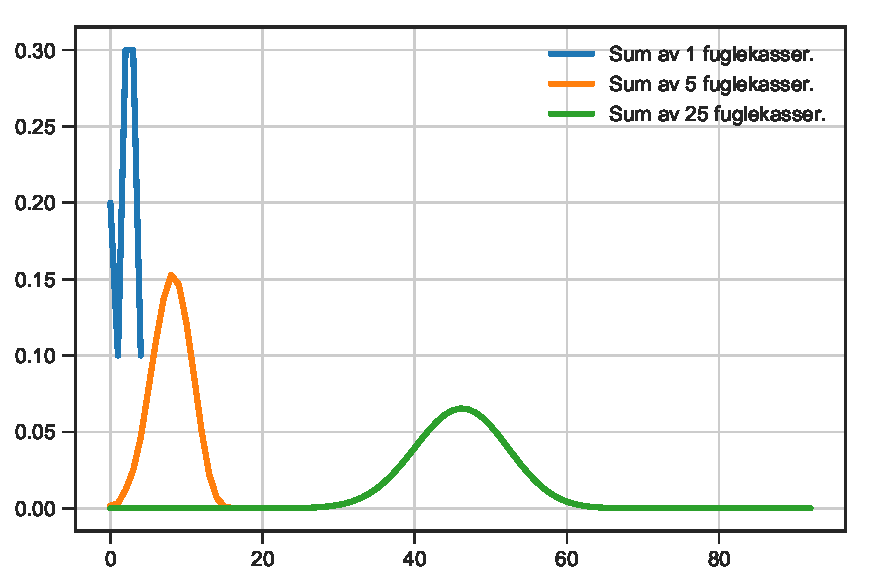
\includegraphics[width=0.65\linewidth]{figs/fuglekasser.pdf}
		\caption{Summen av stokastiske variabler blir normalfordelt, oppgave 6c, del 1. }
		\label{fig:fuglekasser}
	\end{figure}
	
	
	# Vi kan gjøre utregningene som dette:
	\begin{align*}
		\operatorname{E}(S) &= \operatorname{E}\left(X_1 + X_2 + \dots + X_n\right) \\
		&= \operatorname{E}(X_1) + \operatorname{E}(X_2) + \dots +  \operatorname{E}(X_n) = n \operatorname{E}(X) = n\mu = 100(2) = \answer{200} \\
		\operatorname{Var}(S) &= \operatorname{Var}\left(X_1 + X_2 + \dots + X_n\right) \\
		&= \operatorname{Var}(X_1) + \operatorname{Var}(X_2) + \dots +  \operatorname{Var}(X_n) = n \operatorname{Var}(X) \\ &= n \sqrt{1.6}^2 = 100(1.6) = \answer{160}
	\end{align*}
	Eller vi kan bruke formlene $\mu_S = n \mu_X$ og $\sigma_S^2 = n \sigma_X^2$ direkte.
	Vi får samme svar uansett.
	
	# Her må vi bruke $Z = (S-\mu)/\sigma$ for å transformere vår normalfordelte $S$
	til en standardnormalfordelt $Z$ med $\mu_Z = 0$ og $\sigma_Z = 1$. Vi regner slik:
	\begin{align*}
		P(S \geq 226) &= 1 - P(S < 226) \qquad (\text{snu fordi tabellen gir }P(Z \leq z)) \\
							&= 1 - P \left(\frac{S-\mu}{\sigma} < \frac{226-\mu}{\sigma}\right) \\
							&= 1 - P \left(Z < \frac{226-200}{13}\right) \\
							&= 1 - P \left(Z < 2\right) \\
							&= 1 - 0.9772  \qquad (\text{fra tabell})\\
							&= 0.0228 \approx 2.3 \%
	\end{align*}
	Det er altså en \answer{2.3 \%} sannsynlighet for at 226, eller flere, kjøttmeisunger overlever.\footnote{For å få helt riktig svar må vi korrigere for heltallene. Vi bruker en kontinuerlig fordeling til å approksimere en diskret funksjon. Det blir nok enda mer nøyaktig å regne $P(S \geq 226)^{(\text{diskret})} \cong P(S \geq 225.5)^{(\text{kontinuerlig})} = 0.02490812 \approx 2.5 \%$. Dette er bare en kommentar. På del 1 handler det også om å få greie verdier som man kan slå opp i tabellen.}
	# Vi kan regne som dette:
	\begin{align*}
		P(187 \leq S \leq 213) &= P(S \leq 213) - P(S \leq 187) \\
		&= P \left(\frac{S-\mu}{\sigma} \leq \frac{213-\mu}{\sigma}\right) - 
		P \left(\frac{S-\mu}{\sigma} \leq \frac{187-\mu}{\sigma}\right) \\
		&= P \left(Z \leq \frac{213-200}{13}\right) - 
		P \left(Z \leq \frac{187-200}{13}\right) \\
		&= P \left(Z \leq 1\right) - 
		P \left(Z \leq -1\right) \\
		&= 0.8413 - 
		0.1587 =  0.6827 \approx \answer{68.3\%}
	\end{align*}
\end{easylist}



	
\pagebreak
\section*{Del 2 - med hjelpemidler}

\subsection*{Oppgave 1}
\begin{easylist}[enumerate]
	\ListProperties(Style2*=,Numbers=a,Numbers1=l,FinalMark={)})
	# Hver setning gir oss én likning:
	\begin{easylist}[itemize]
		## ``\textbf{Når bedriften produserer 200 enheter per uke, blir overskuddet lik 0.}'' \\
		\begin{equation*}
			O(200) = 0 \quad \Rightarrow \quad O(200) = a (200)^2 + b(200) + c = 0 \quad \Rightarrow \quad 40000a + 200b + c = 0
		\end{equation*}
		## ``\textbf{Overskuddet er størst når bedriften selger 475 enheter.}''\\
		Da er $O'(475) = 0$. Vi har at $O'(x) = 2ax + b$, og får:
		\begin{equation*}
		O'(475) = 0 \quad \Rightarrow \quad O'(475) = 2a (475) + b = 0 \quad \Rightarrow \quad 950a + b = 0
		\end{equation*}
		## ``\textbf{Når bedriften selger 600 enheter per uke, er grensekostnaden 5 kroner større enn grenseinntekten.}'' \\
		Fra setningen ovenfor får vi vite at $K'(600) = I'(600) + 5$. Definisjonen av overskudd sier at $O'(600) = I'(600) - K'(600)$. Når vi setter inn det vi får vite i definisjonen, får vi
		$O'(600) = I'(600) - \left(I'(600) + 5\right) = -5$.
		\begin{equation*}
		O'(600) = -5 \quad \Rightarrow \quad O'(600) = 2a (600) + b = -5 \quad \Rightarrow \quad 1200a + b = -5
		\end{equation*}
	\end{easylist}
	Vi får altså likningsystemet:
	\begin{align}
		\nonumber 40000a + 200b + c &= 0 \\
		\label{eqn:system}950 a + b &= 0 \\
	\nonumber	1200a + b &= -5
	\end{align}
	Som var det oppgaven ba oss om å vise.
	# Vi skriver likningssystem \eqref{eqn:system} inn i CAS slik: \\
	\verb|NLøs[{40000a + 200b + c = 0, 950a + b = 0, 1200a + b = -5}, {a, b, c}]|
	Og vi får vite at \answer{$a = -0.02$, $b = 19$ og $c = -3000$}.
	
	# Vi plotter funksjonen ved hjelp av \\
	\verb|O(x) = -0.02*x*x + 19x -3000| \\
	i Geogebra. For å finne maksimumspunktet skriver vi inn \\
	\verb|Maks[O, 0, 800]| \\
	Vi får vite at maksimumspunktet er $(475, 1512.6)$.
	Det største overskuddet bedriften kan få per uke er altså \answer{1512.6}.
\end{easylist}



\subsection*{Oppgave 2}
\begin{easylist}[enumerate]
	\ListProperties(Style2*=,Numbers=a,Numbers1=l,FinalMark={)})
	# Her kan det være lurt å lage en tabell og lete etter et mønster.
	Vi kaller bankinnskuddet for $b$, slik at $b = 20000$ i denne oppgaven.
	Videre kaller vi renten for $r$, altså er $r = 1.03$ i denne oppgaven.
	\begin{center}
		\begin{tabular}{lll}
			\textbf{År} & \textbf{Antall år etter start} ($n$) & \textbf{Penger på konto} ($P_n$) \\ \hline
			2018 & 0 & $b$ \\
			2019 & 1 & $br + b$ \\
			2020 & 2 & $b(r^2 + r + 1)$ \\
			$\vdots$ & $\vdots$ & $\vdots$ \\
			2052 & 34 & $b \left(r^{34} + r^{33} + \dots + r^2 + r + 1\right)$
		\end{tabular}
	\end{center}
	

	Dersom $P_n$ er penger etter $n$ år, så er den rekursive regelen
	at $P_n = P_{n-1}r + b$, altså ``pengene i år er pengene fra forrige år, ganget med renten, pluss et nytt bankinnskudd.''
	Generelt får vi at $P_n = b \left(r^{n} + r^{n-1} + \dots + r^2 + r + 1\right)$.
	Når vi setter inn $n = 34$, $b = 20000$ og $r = 1.03$ får vi
	\begin{equation*}
		P_{34} = 20000 \left(1.03^{34} + 1.03^{33} + \dots + 1.03^2 + 1.03 + 1\right) = b \sum_{i=0}^{34} r^i
	\end{equation*}
	I Geogebra gjør vi som vist i figur \ref{fig:cas1}. Svaret blir $\answer{1209242}$.
	
	\begin{figure}[th!]
		\centering
		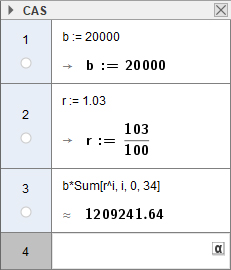
\includegraphics[width=154px]{figs/v17_2a_del2.jpg}
		\caption{Skjermbilde fra CAS for oppgave 2a, del 2.}
		\label{fig:cas1}
	\end{figure}
	# Igjen kan det være nyttig å sette opp en tabell.
	Vi lar $I = 1209242$ være innskuddet som Ingrid har spart opp i 2052. Vi antar at Ingrid har pengene på samme konto fra 2052 til 2053, og lar $r = 1.03$ være renten og $u$ være det ukjente uttaket.
		\begin{center}
		\begin{tabular}{lll}
			\textbf{År} & \textbf{År etter første uttak} ($n$) & \textbf{Penger på konto} ($P_n$) \\ \hline
			2052 & -1 & $I$ \\
			2053 & 0 & $Ir - u$ \\
			2054 & 1 & $Ir^2 - u(r+1)$ \\
			2055 & 2 & $Ir^3 - u(r^2 + r+1)$ \\
			$\vdots$ & $\vdots$ & $\vdots$ \\
			2067 & 14 & $Ir^{15} - u (r^{14} + r^{13} + \dots + r^2 + r + 1)$
		\end{tabular}
	\end{center}
	Den rekursive regelen er lik den forrige, men nå tar vi ut $u$ hvert år. Regelen er $P_n = P_{n-1}r - u$. Kontoen skal være tom etter 14 år, så vi løser
	\begin{equation*}
		P_{14} = Ir^{15} - u (r^{14} + r^{13} + \dots + r^2 + r + 1) = Ir^{15} - u \sum_{i = 0}^{14} r^i = 0
	\end{equation*}
	I Geogebra løser vi som vist på figur \ref{fig:cas2}. Svaret blir $\answer{101294}$.
	\begin{figure}[th!]
		\centering
		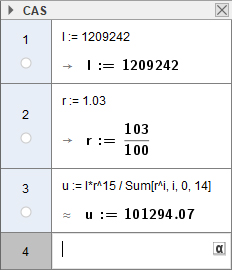
\includegraphics[width=154px]{figs/v17_2b_del2.jpg}
		\caption{Skjermbilde fra CAS for oppgave 2b, del 2.}
		\label{fig:cas2}
	\end{figure}
	

	# Fra forrige oppgave vet vi at
	\begin{equation*}
		P_{n} = Ir^{n+1} - u (r^{n} + r^{n-1} + \dots + r^2 + r + 1) = Ir^{n+1} - u \sum_{i = 0}^{n} r^i
	\end{equation*}
	der $n$ er antall år etter 2053.
	Vi løser $P_n = 0$ som vist i figur \ref{fig:cas3}.
	\begin{figure}[th!]
		\centering
		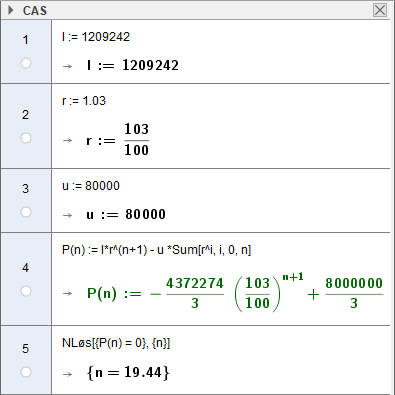
\includegraphics[width=263px]{figs/v17_2c_del2.jpg}
		\caption{Skjermbilde fra CAS for oppgave 2c, del 2.}
		\label{fig:cas3}
	\end{figure}
	Kontoen er tom $19.44$ år etter 2053, altså i år $2072.44$.
	Oppgaven spør når kontoen vil være tom:
	man vil kunne ta ut et fullt uttak i 2072, men i 2073 vil man bare kunne ta 
	ut et ufullstendig uttak på 34395 kroner som vil tømme kontoen. Kontoen vil 
	tømmes i \answer{2073}.
\end{easylist}


\subsection*{Oppgave 3}
\begin{easylist}[enumerate]
	\ListProperties(Style2*=,Numbers=a,Numbers1=l,FinalMark={)})
	# La $X = \mathcal{N}(\mu = 30, \sigma = 3)$ være levetiden til  et tilfeldig valg batteri.
	Vi kan bruke sannsynlighetskalkulatoren i Geogebra, som er raskt og enkelt. Her viser jeg hvordan oppgaven kan regnes ut
	ved hjelp av standardnormalfordelingstabellen:
	\begin{align*}
		P(X < 27) &= P\left( \frac{X - \mu}{\sigma} < \frac{27 - \mu}{\sigma} \right) \\
		&= P\left( Z < \frac{27 - 30}{3} \right) \\
		&= P\left( Z < -1 \right) \\
		&=\answer{ 0.1587} 
	\end{align*}
	
	# La $Y$ være forventet levetid for batteriene, altså gjennomsnittlig levetid for batteriene. Levetiden til et batteri er en stokastisk variabel $X = \mathcal{N}(\mu = 30, \sigma = 3)$, og levetiden til gjennomsnittet er da gitt ved $Y = \mathcal{N}(\mu_Y = 30, \sigma_Y = \sigma / \sqrt{n})$. Vi setter opp hypotesene slik:
	\begin{align*}
		H_0 : \quad & Y = 30 \\
		H_1 : \quad & Y < 30 
	\end{align*}
	Den observerte verdien for $Y$, her kalt $Y_{\text{obs}}$, blir er:
	\begin{equation*}
		Y_{\text{obs}} = \frac{29+31+32+27+29+25+23+30+26}{9} = 28
	\end{equation*}
	La oss bruke $p$-verdien til å trekke en konklusjon. $p$-verdien er sannsynligheten for noe like ekstremt, eller mer ekstremt, som den observerte $Y_{\text{obs}}$, gitt at $H_0$ er sann.
	Dersom $H_0$ er sann er $Y$ normalfordelt med forventing $\mu_Y = 30$ og $\sigma_Y = \sigma / \sqrt{n} = 3 /\sqrt{9} = 1$.
	\begin{align*}
		p\text{-verdi} &= P(Y <Y_{\text{obs}} | H_0 \text{ er sann}) = P(Y < 28) \\
		&= P\left( \frac{Y-\mu_Y}{\sigma_Y} < \frac{28-30}{1} \right) \\
		&= P\left( Z < -2 \right) \\
		&= 0.0228
	\end{align*}
	Gitt at $H_0$ er sann er det altså $2.28\%$ sannsynlig å trekke ut batterier
	slik at $Y <Y_{\text{obs}}$. Ettersom $p$-verdien er lavere enn $\alpha = 0.05$
	så \answer{forkaster vi $H_0$}.
\end{easylist}


\subsection*{Oppgave 4}
\begin{easylist}[enumerate]
	\ListProperties(Style2*=,Numbers=a,Numbers1=l,FinalMark={)})
	# Vi legger dataene inn i regnearket i Geogebra, deretter markerer vi og trykker  ``Regresjonsanalyse'' oppe til venstre. Vi velger 
	``logistisk regresjon''. Se figur \ref{fig:cas4} for et skjermbilde.
	Svaret blir \answer{$N = 10095$, $a = 49.5$ og $k = 0.50$}.
	\begin{figure}[th!]
		\centering
		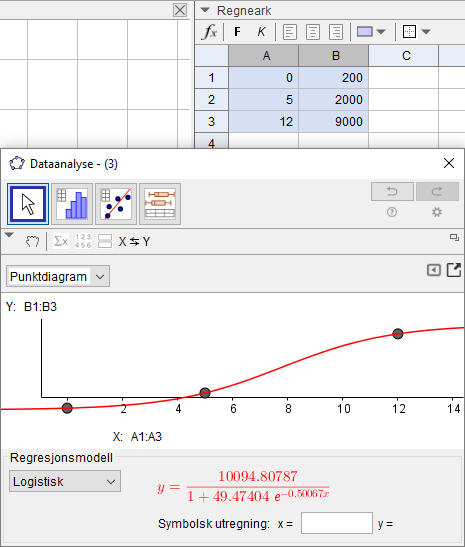
\includegraphics[width=310px]{figs/v17_4a_del2.jpg}
		\caption{Skjermbilde fra CAS for oppgave 4a, del 2.}
		\label{fig:cas4}
	\end{figure} 

	# Vi skriver inn funksjonen $f(x) = 10000 / (1 + 50 e^{-0.5x})$ i Geogebra med kommandoen \\
	\verb|f(x) = 10000 / (1 + 50e^(-0.5*x))| \\
	Deretter laget vi en linje \verb|y = 7000| og velger ``Punkt $\to$ Skjæring mellom to objekt''
	for å få punktet $(9.518, 7000)$. Antall smittede personer per uke er 7000 etter \answer{9.5 uker}, altså passerer vi 7000 smittede i uke 9 etter at sykdommen brøt ut.
	 
	# Bruk kommandoen \verb|I = Integral[f, 0, 12]|. Integralet blir $43700.25$.
	Integralet av en funksjon er ``summen av funksjonen.'' Tolkningen her er at
	integralet er summen av antall smittede per uke, summert fra uke 0 til uke 12, altså totalt antall smittete i perioden.
	\begin{equation*}
		\int_{0}^{12} \underset{\text{smittede / uke}}{\underbrace{f(t)}} \ \underset{\text{uke}}{\underbrace{dt}} = \text{totalt antall smittede fra uke 0 til uke 12} = \answer{43700}
	\end{equation*}
	# Vi løser likningen
	\begin{equation*}
		\int_{0}^{T} f(t) \ dt = 15 000
	\end{equation*}
	for den ukjente $T$ ved \verb|NLøs[{Integral[f, 0, T] = 15000}, {T}]|
	i CAS, og vi får $T = 8.12$ som svar. Det tar rett \answer{over $8$ uker} før 15000 personer
	er smittet totalt.
\end{easylist}
	
	
\end{document}


